\documentclass[../psets.tex]{subfiles}

\pagestyle{main}
\renewcommand{\leftmark}{Problem Set \thesection}

\begin{document}




\section{Working with NMR Spectra}
\begin{enumerate}
    \item \marginnote{2/19:}One of the directories in the 5.46\_NMR\_data folder is called `glucose2\_320mM'; inside this directory are a number of datasets which were acquired at different times or using different NMR experiments.
    \begin{enumerate}
        \item This dataset was, surprisingly, generated from a \SI{320}{\milli\molar} sample of glucose. Glucose exists as a mixture of $\alpha$- and $\beta$-anomers. Draw the structures of each in chair form, and label each anomer.
        \begin{proof}
            {\color{white}hi}
            \begin{figure}[H]
                \centering
                \footnotesize
                \begin{subfigure}[b]{0.25\linewidth}
                    \centering
                    \chemfig[fixed length=false]{(-[:-160]HO)-[:-10](-[:130]-[:70]OH)-[:20]O-[:-50](-[6]OH)-[:170](-[:-50,,,2]HO)-[:-160](-[:170,0.8]HO)-[:130]}
                    \caption{$\alpha$-D-glucose.}
                \end{subfigure}
                \begin{subfigure}[b]{0.25\linewidth}
                    \centering
                    \chemfig[fixed length=false]{(-[:-160]HO)-[:-10](-[:130]-[:70]OH)-[:20]O-[:-50](-[:20]OH)-[:170](-[:-50,,,2]HO)-[:-160](-[:170,0.8]HO)-[:130]}
                    \caption{$\beta$-D-glucose.}
                \end{subfigure}
            \end{figure}
        \end{proof}
        \item Find experiment \#4, load it into MestReNova or TopSpin, and generate a properly phased spectrum. Use the software to integrate the peaks or regions, and expand the spectrum to include only the region around water to include the anomeric protons.
        \begin{proof}
            {\color{white}hi}
            \begin{center}
                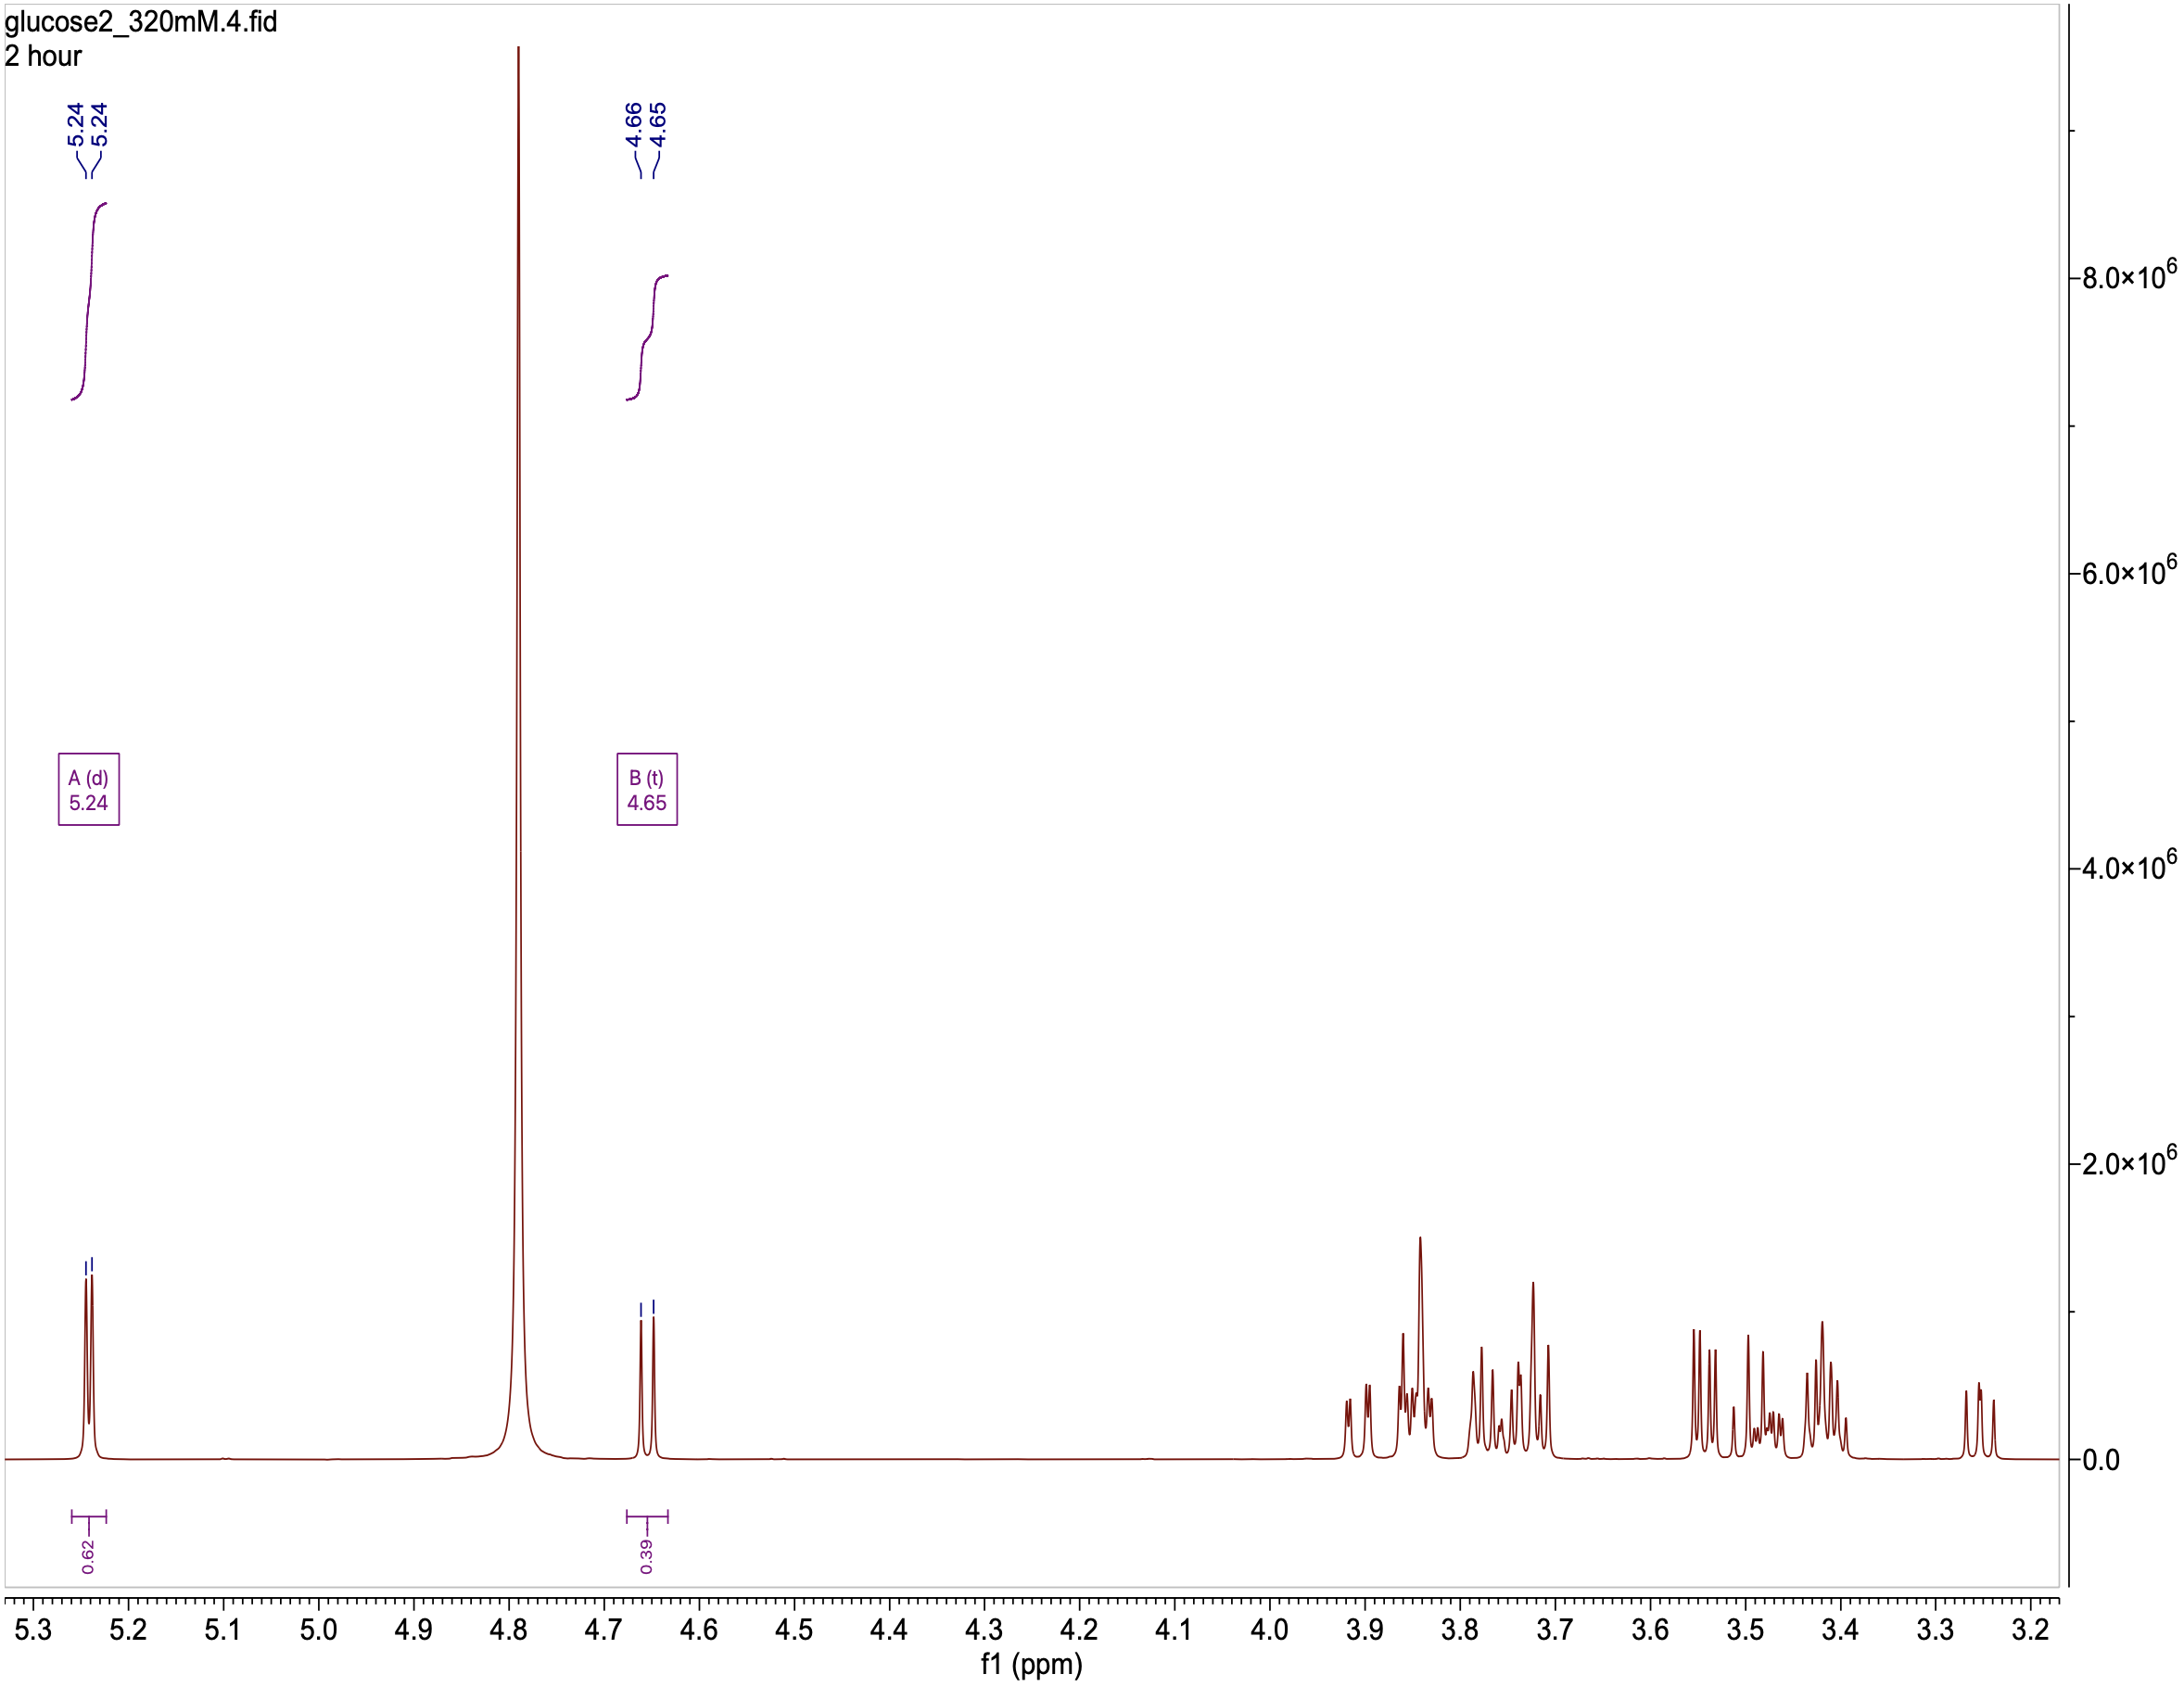
\includegraphics[width=\linewidth]{PSet1Q1b.png}
            \end{center}
        \end{proof}
        \item Measure the ${}^3J_{\ce{HH}}$ coupling constant and the ${}^1J_{\ce{CH}}$ coupling constant for each anomeric proton. Make a table showing the chemical shift for each anomeric proton, the relative integrals (which should total 100\%), and the two coupling constants.
        \begin{proof}
            {\color{white}hi}
            \begin{table}[H]
                \centering
                \small
                \renewcommand{\arraystretch}{1.2}
                \begin{tabular}{c|cccc}
                    \textbf{Pyranose} & \textbf{Chemical Shift} & \textbf{Integral} & $\bm{{}^3J_{\ce{HH}}}$ & $\bm{{}^1J_{\ce{CH}}}$\\
                    \hline
                    $\alpha$-D-glucose & \SI{5.24}{\partspermillion} & 61\% & \SI{3.81}{\hertz} & \SI{169.50}{\hertz}\\
                    $\beta$-D-glucose  & \SI{4.65}{\partspermillion} & 39\% & \SI{7.96}{\hertz} & \SI{164.62}{\hertz}\\
                \end{tabular}
            \end{table}
        \end{proof}
        \item Using the fact that the $\beta$-anomer is expected to be about 60\% of the total, rationalize the variation in chemical shift and coupling constants for each.
        \begin{proof}
            Contrary to the expected integrals, the peak characteristic of the $\alpha$-anomer integrates to approximately 61\% of the total in the provided data file. Perhaps the anomers were taken out of equilibrium before the spectrum was taken and are in the process of reequilibrating.\par
            Regardless, the $\beta$-anomer's anomeric proton should be more shielded because of the anomeric effect's no-bond resonance placing a $\delta^-$ on that proton; such resonance does not occur in the $\alpha$-anomer. This effect is clearly observed, as the $\beta$-anomer's doublet is \SI{0.59}{\partspermillion} upfield from the $\alpha$-anomer's doublet. Note that the downfield doublets were originally identified as the anomeric peaks because the anomeric protons should be the most deshieleded due to their position on the glucose hemiacetal (the position nearest to the most electron-withdrawing hydroxyl groups).\par
            Additionally, the $\beta$-anomer's ${}^3J_{\ce{HH}}$ coupling constant should be larger than the $\alpha$-anomer's due to the Karplus correlation. Indeed, the $\beta$-anomer's anomeric proton is oriented antiperiplanar to the C2 proton, while the $\alpha$-anomer's anomeric proton is oriented gauche. This effect is also clearly observed, as the $\beta$-anomer has a ${}^3J_{\ce{HH}}$ value \SI{4.15}{\hertz} greater than the $\alpha$-anomer's ${}^3J_{\ce{HH}}$ value.\par
            Lastly, the $\beta$-anomer's ${}^1J_{\ce{CH}}$ coupling constant should be smaller than the $\alpha$-anomer's because the relevant \ce{C-H} bond is longer in the $\beta$-anomer. This bond elongation is again a result of the anomeric effect, specifically $n_{\ce{O}}\to\sigma^*_{\ce{CH}}$ donation. This effect is again observed, as the $\beta$ anomer has a ${}^1J_{\ce{CH}}$ value \SI{4.88}{\hertz} smaller than the $\alpha$-anomer's ${}^1J_{\ce{CH}}$  value.
        \end{proof}
    \end{enumerate}
    \item A second directory in the data folder is called `glucose1\_320mM'; this sample is also glucose at \SI{320}{\milli\molar} with one difference -- this glucose is fully \ce{{}^13C} labeled. Analyze the anomeric region of spectrum \#4 in the same way as you did for the first sample. Explain the difference in apparent anomeric ratio as best you can.
    \begin{proof}
        {\color{white}hi}
        \begin{table}[H]
            \centering
            \small
            \renewcommand{\arraystretch}{1.2}
            \begin{tabular}{c|cccc}
                \textbf{Pyranose} & \textbf{Chemical Shift} & \textbf{Integral} & $\bm{{}^3J_{\ce{HH}}}$ & $\bm{{}^1J_{\ce{CH}}}$\\
                \hline
                $\alpha$-D-glucose & \SI{5.24}{\partspermillion} & 62\% & ?? & \SI{169.92}{\hertz}\\
                $\beta$-D-glucose  & \SI{4.65}{\partspermillion} & 39\% & ?? & \SI{165.08}{\hertz}\\
            \end{tabular}
        \end{table}
        Of note is that the central chemical shift values do not change (as expected), and the coupling constants only increase marginally (perhaps insignificantly). The ${}^1J_{\ce{CH}}$ values are also difficult to measure --- especially for the $\alpha$-anomer --- because of the appearance of apparently new couplings that split the peaks into pseudo-quartets.\par
        Additionally, there does not appear to be a significant difference in the anomeric ratio. Rather, the $\alpha:\beta$ ratio appears to be approximately $62:38$ instead of $61:39$.
    \end{proof}
    \item For the spectra you have been working with, measure the amount of water relative to the glucose. Estimate the amount of water, and think about where this water signal comes from. Which glucose sample has more water in it?
    \begin{proof}
        The residual solvent peak at \SI{4.79}{\partspermillion} in glucose2\_320mM.4.fid integrates to 3.82 times the height of the sum of the anomeric peaks. This means that for each glucose anomeric proton in solution, there are 3.82 water protons. Since there is one glucose anomeric proton per glucose molecule but two water protons per molecule, it follows that there are 1.91 water molecules for each glucose molecule in solution. Thus, the concentration of water in this sample is
        \begin{equation*}
            1.91\times\SI{320}{\milli\molar} = \SI{611}{\milli\molar}
        \end{equation*}\par
        By an analogous calculation, the concentration of water in glucose1\_320mM.4.fid is
        \begin{equation*}
            2.01\times\SI{320}{\milli\molar} = \SI{643}{\milli\molar}
        \end{equation*}
        Thus, \fbox{glucose1\_320mM.4.fid has more water in it.} The water signal most likely comes partially from leftover \ce{H2O} contamination in the isotopically enriched \ce{D2O} solvent, and partially from proton-deuterium exchange between \ce{D2O} and undeuterated glucose.
    \end{proof}
\end{enumerate}




\end{document}